% Per presentazione
\documentclass{beamer}

\graphicspath{{img/}}
\usepackage{multicol}

%Per stampare senza animazioni:
%\documentclass[handout]{beamer}

% Per stampare più slides per pagina
%\usepackage{pgfpages}
%\pgfpagesuselayout{4 on 1}[a4paper, landscape, border shrink=5mm]		%vedi file presentazione_handout_4on1
%\pgfpagesuselayout{2 on 1}[a4paper, portrait, border shrink=5mm]		%vedi file presentazione_handout_2on1
%\nofiles


\usetheme{SUPSI}


\titolo{SaniWiki}
\studente{Maura Clerici\\Antonio Daniele Mu}
\relatore{Riccardo Mazza}

\committente{Lara Barro\\DEASS SUPSI}
\corso{Ing. informatica}
\anno{2018-2019}
% se si vuole una data fissa
\data{7 febbraio, 2019}
% Se si vuole la data corrente, mettere:
%\data{ \today}



\begin{document}

\makeatletter
    \newenvironment{withoutfootline}{
        \setbeamertemplate{footline}[default]
        \def\beamer@entrycode{\vspace*{\footheight}}
    }{}
\makeatother


% Per aggiungere una pagina di titolo prima delle nuove sezioni
\AtBeginSection[] { 
  \begin{frame}
	\mysectionpage
  \end{frame} 
} 


\maketitle
\begin{frame}{Indice}
   \tableofcontents
 
\end{frame}

% --------------------------------------------------------------------------

\section{Introduzione}
\begin{frame}{Problema attuale}
	 \begin{itemize}
	\item Centralizzazione dei documenti
	\item Condivisione delle informazioni
\end{itemize}
\end{frame}

% --------------------------------------------------------------------------

\section{Analisi}
\begin{frame}{Utilizzatori}
\begin{itemize}
	\item studenti DEASS
	\item docenti DEASS
\end{itemize}
\end{frame}

\begin{frame}{Situazione attuale - Home page}
\begin{columns}
	\column{1\textwidth}
		\begin{figure}[!h]
			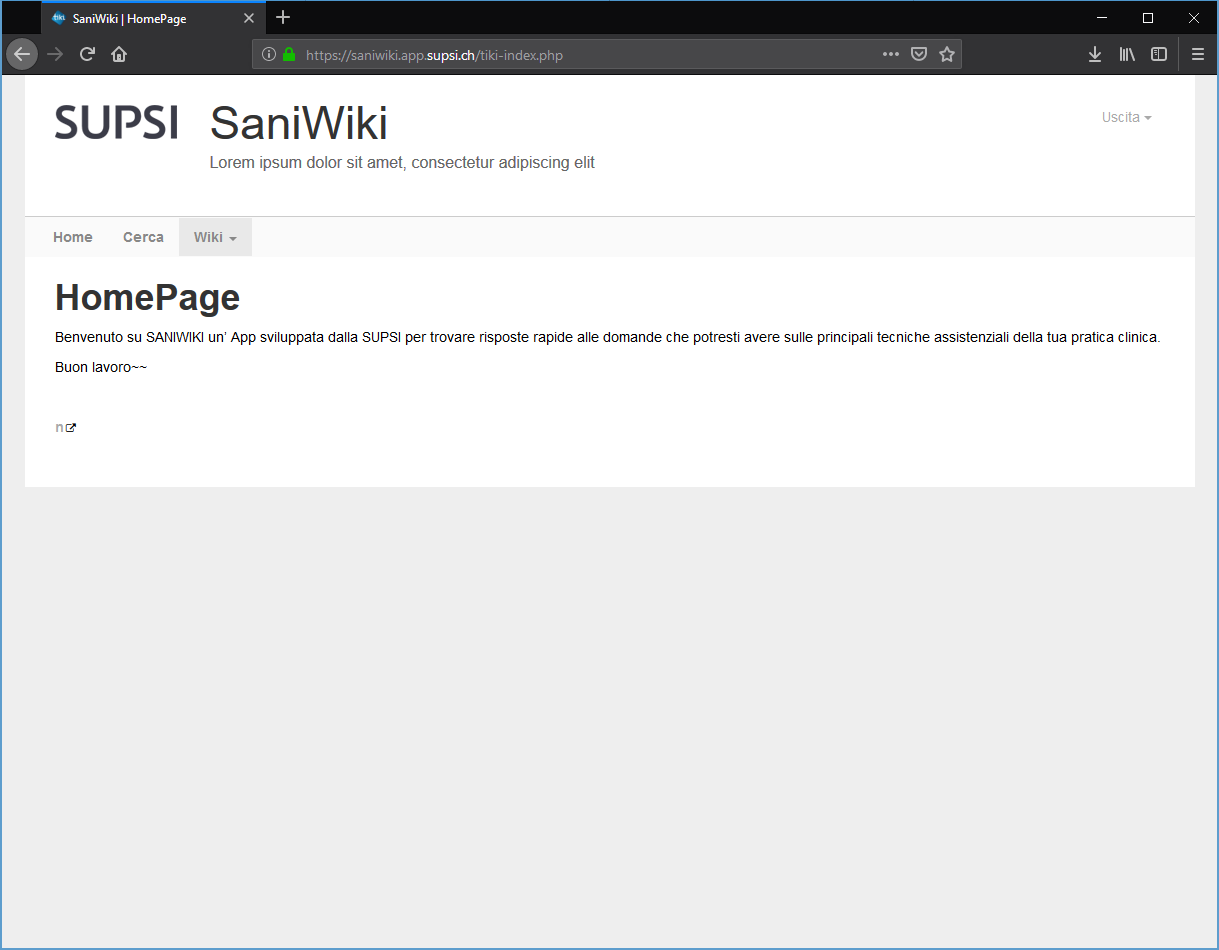
\includegraphics[scale=0.2]{saniold_home.png}
		\end{figure}
\end{columns}
\end{frame}

\begin{frame}{Situazione attuale - Modello di pagina}
\begin{columns}
\column{1\textwidth}
	\begin{figure}[!h]
			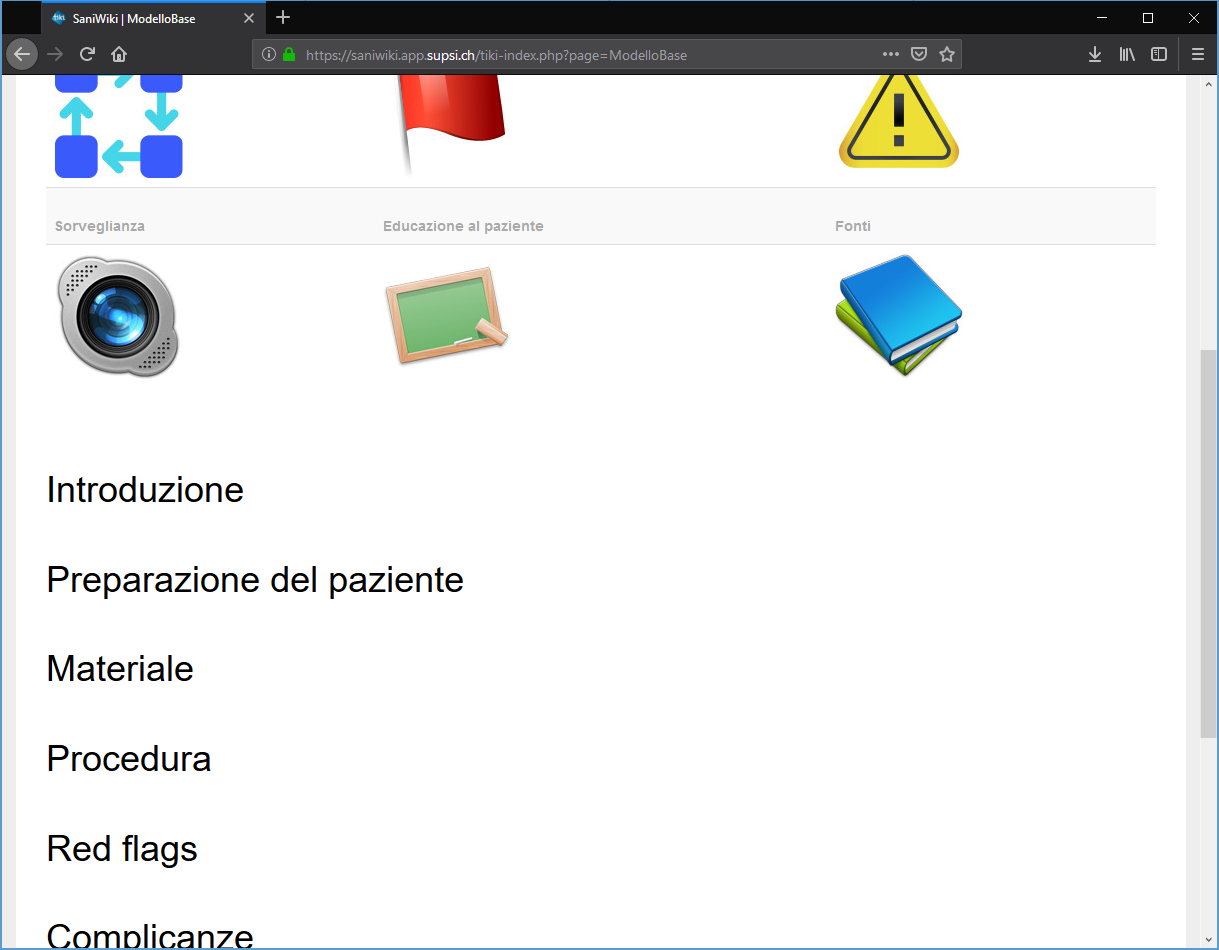
\includegraphics[scale=0.2]{saniold_template.png}
		\end{figure}
\end{columns}
\end{frame}

\begin{frame}{Situazione attuale - Vista articoli}
\begin{columns}
	\column{1\textwidth}
		\begin{figure}[!h]
			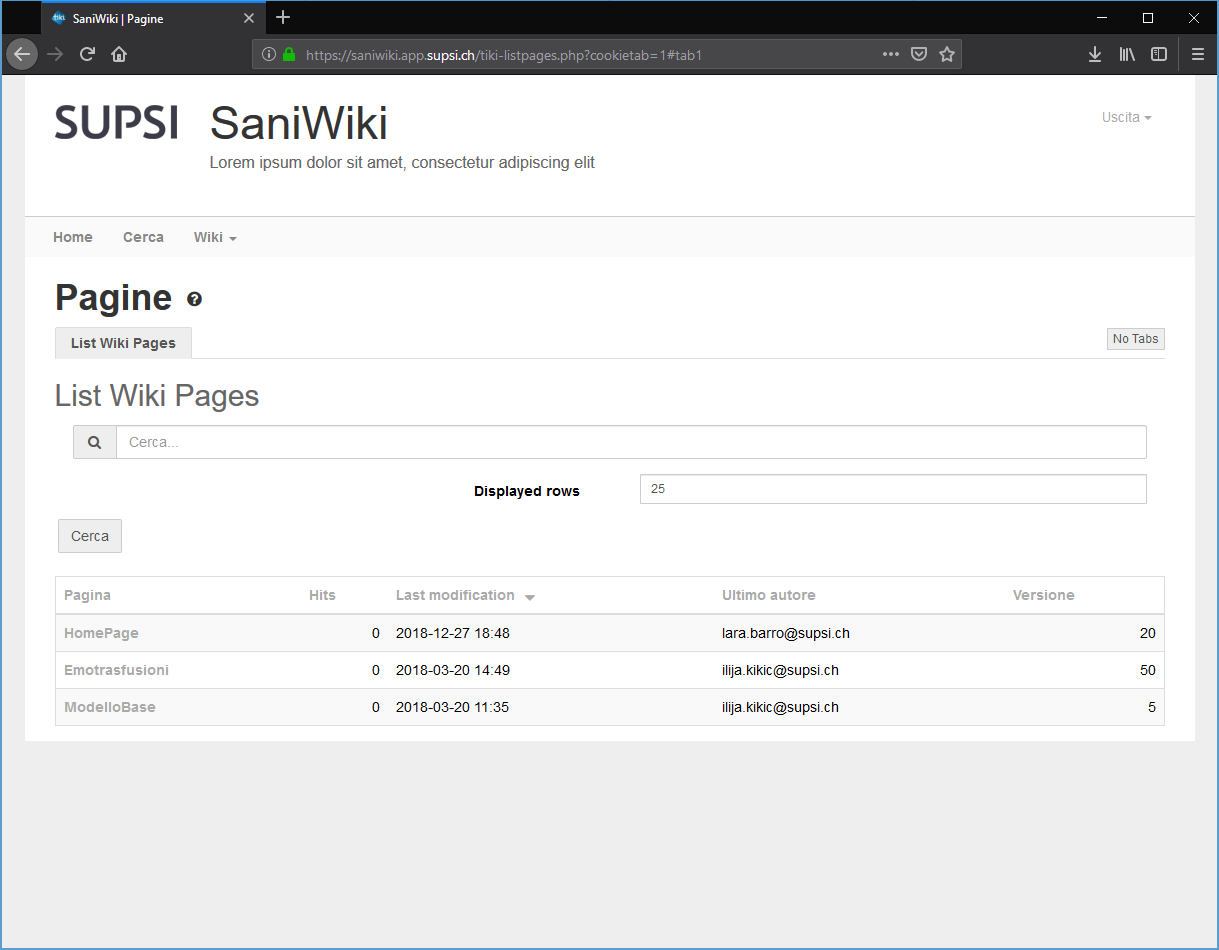
\includegraphics[scale=0.2]{saniold_list.png}
		\end{figure}
\end{columns}
\end{frame}

\begin{frame}{Situazione attuale - Funzione ricerca}
\begin{columns}
\column{1\textwidth}
	\begin{figure}[!h]
			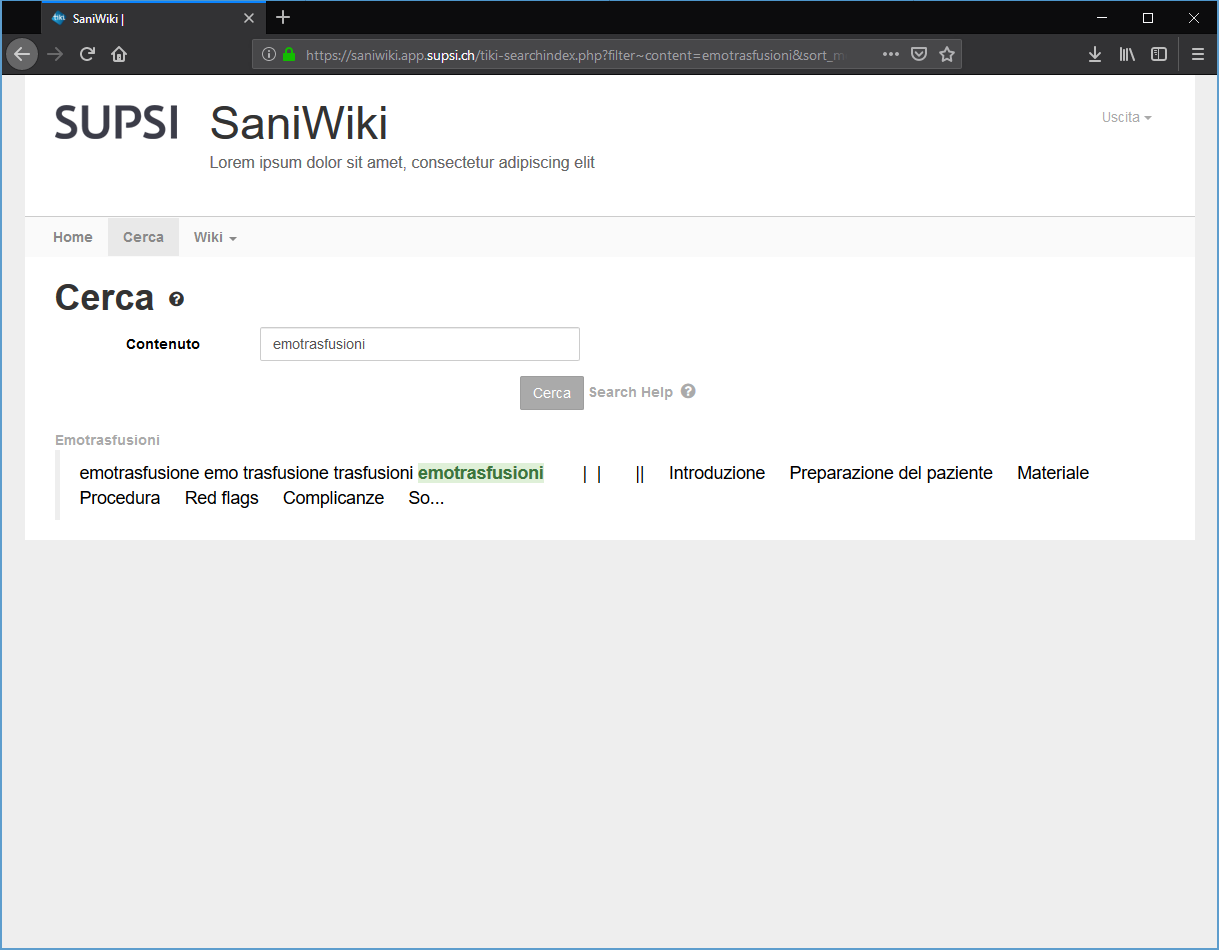
\includegraphics[scale=0.2]{saniold_search.png}
		\end{figure}
\end{columns}
\end{frame}

\begin{frame}{Requisiti}
\setbeamercovered{transparent}
\begin{itemize}
	\item<1-> Compatibilità dispositivi mobili e computer
	\item<2-> Accesso immediato alle risorse
	\item<3-> Suddivisione degli articoli in argomenti
	\item<4-> Controllo ordine di visualizzazione
	\item<5-> Sicurezza sui contenuti
	\item<6-> Immediatezza nel ottenere le informazioni
	\item<7-> Grafica intuitiva
\end{itemize}
\end{frame}

% --------------------------------------------------------------------------

\section{Studio delle Soluzioni}
\begin{frame}{Scelte iniziali}
\begin{columns}
	\column{.5\textwidth}
		\begin{itemize}
		\item Micro framework veloce
		\end{itemize}
		\bigskip
		\bigskip
		\bigskip
		\bigskip
		\begin{itemize}
			\item Mobile App
			\item Potente e versatile
			\item Orientato al design
		\end{itemize}
	\column{.5\textwidth}
	\begin{figure}[!h]
		
\includegraphics[scale=0.25]{lumen-logo.png}
	\end{figure}
	\begin{figure}[!h]
		
\includegraphics[scale=0.1]{ionic-logo.jpg}
	\end{figure}
\end{columns}
\end{frame}

\begin{frame}{Scelte definitive}
\begin{columns}
	\column{.5\textwidth}
		\begin{itemize}
			\item Framework completo
			\item Template engine
			\item Supporto maggiore
			
		\end{itemize}
	\column{.5\textwidth}
	\begin{figure}[!h]
		
\includegraphics[scale=0.04]{Laravel-logo.png}
	\end{figure}
\end{columns}
\end{frame}

\begin{frame}{Tecnologie usate}
	\begin{figure}[!h]
		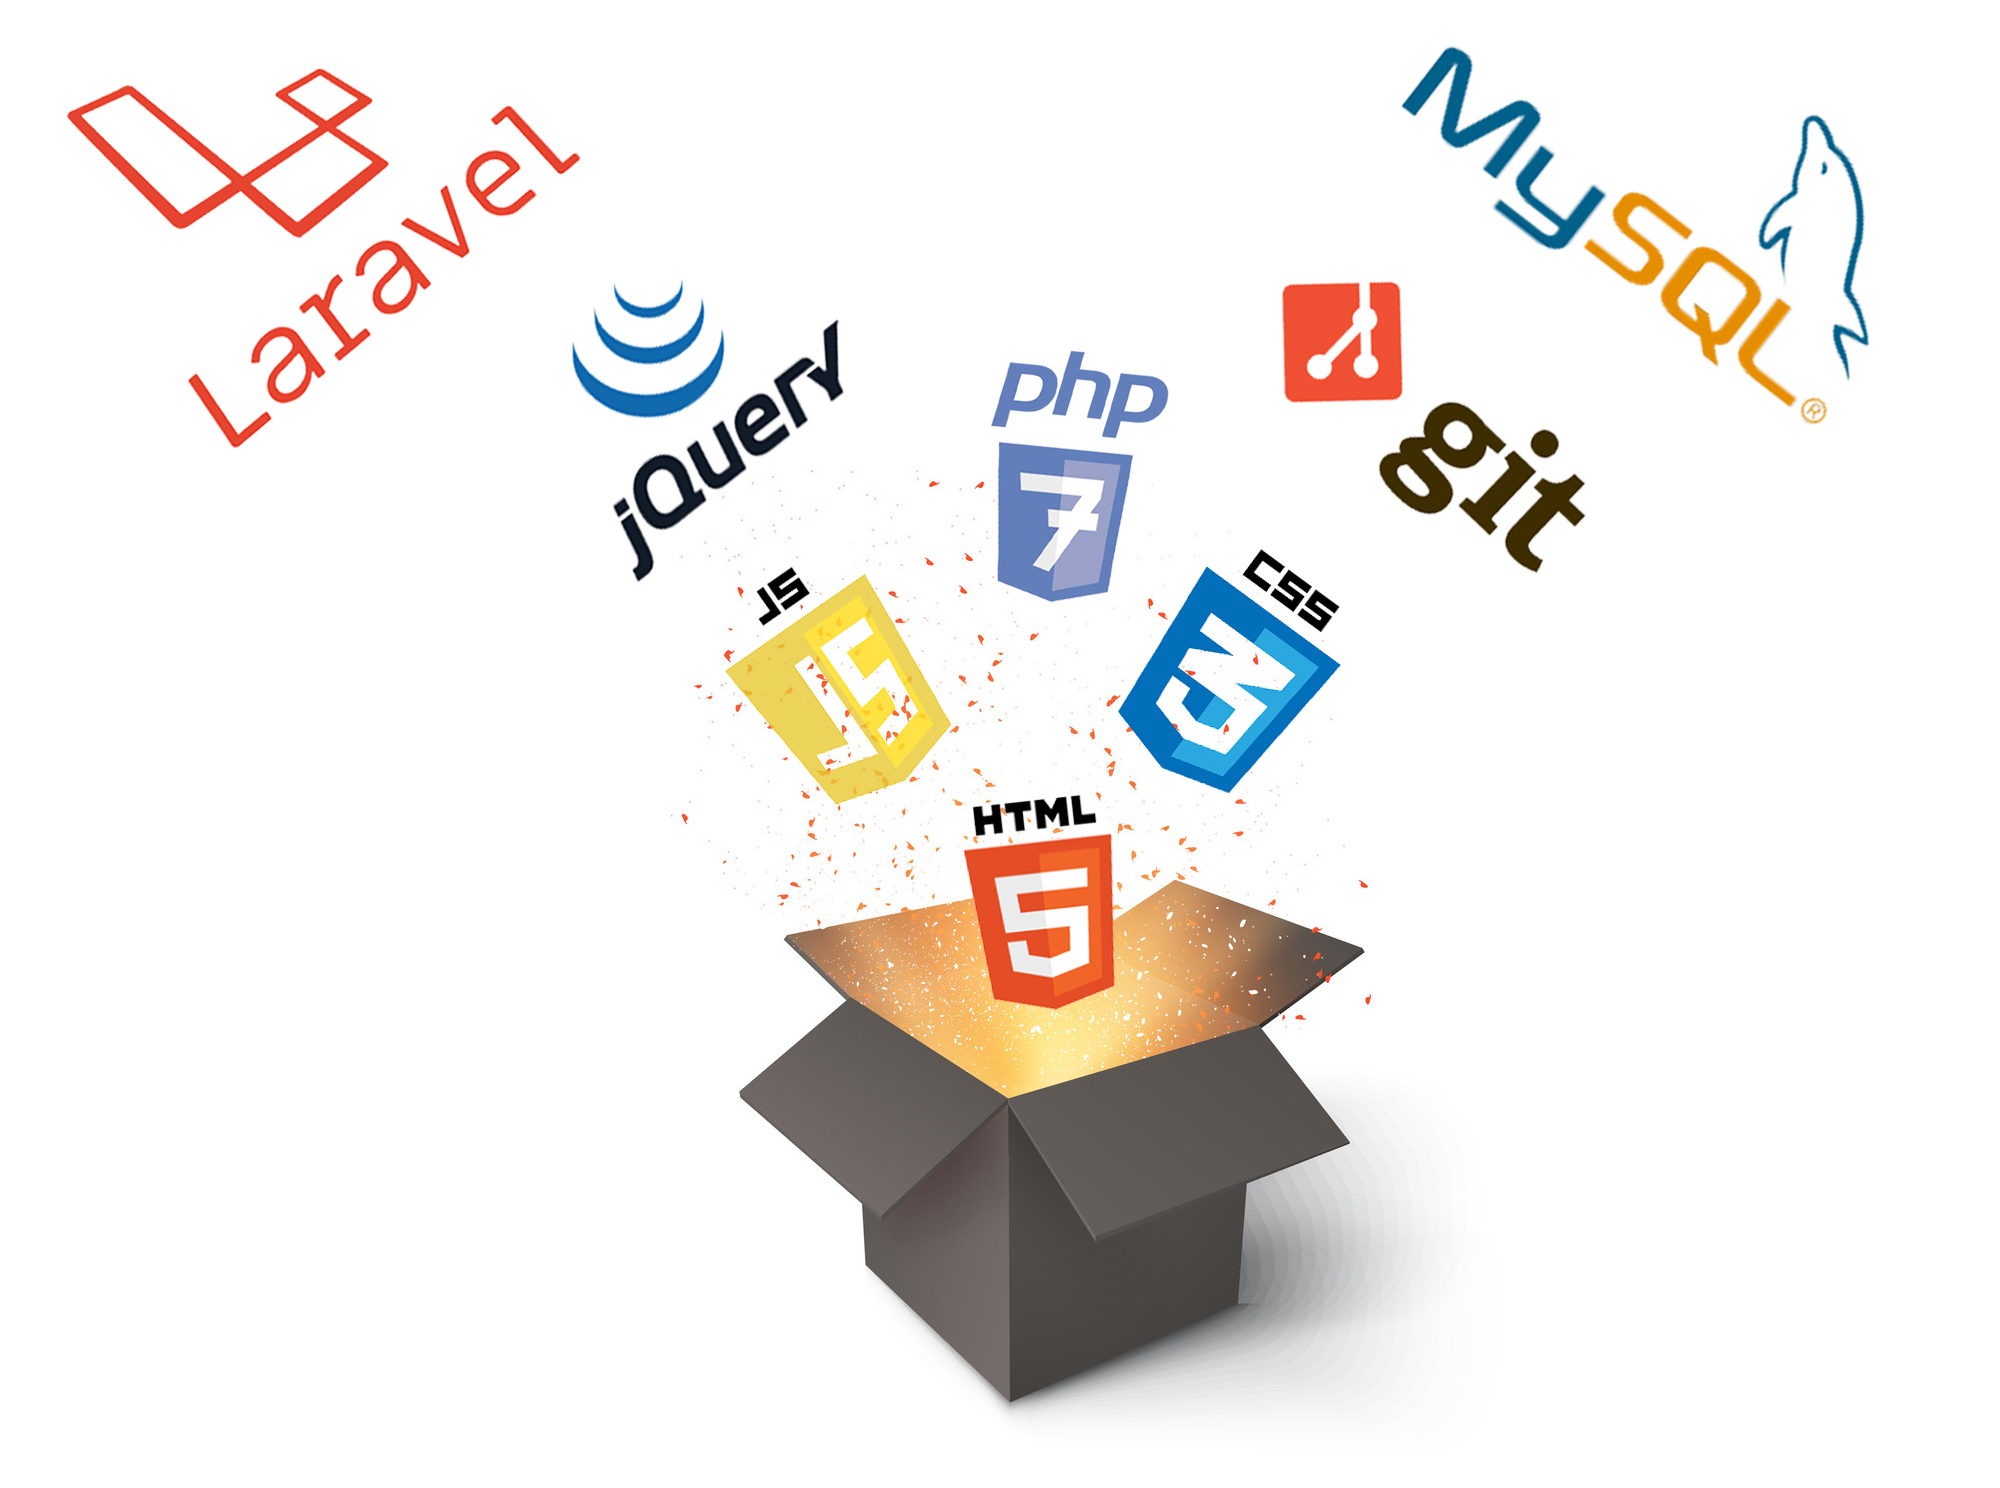
\includegraphics[scale=0.59]{tecnologie.jpg}
	\end{figure}
\end{frame}

% --------------------------------------------------------------------------

\section{Progettazione}
\begin{frame}{Schema della struttura}
	\begin{figure}[!h]
		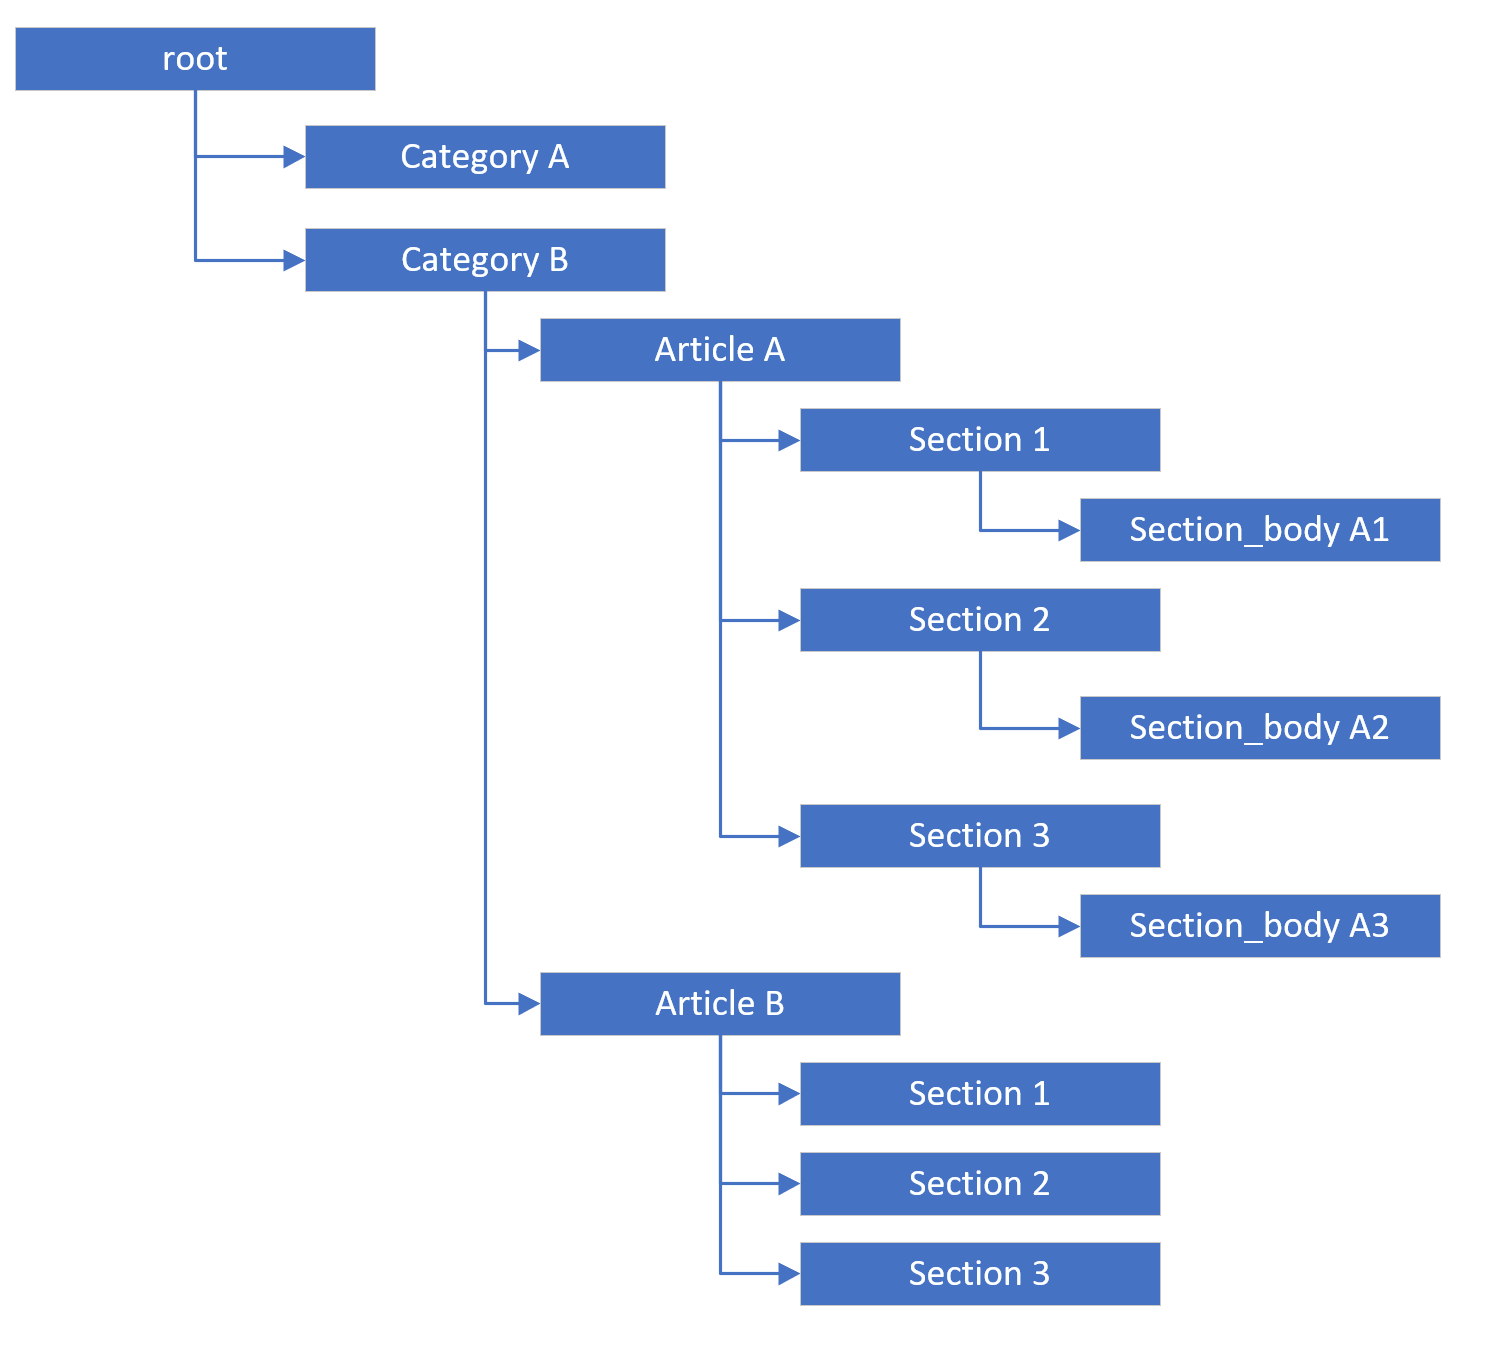
\includegraphics[scale=0.35]{root.png}
	\end{figure}
\end{frame}
\begin{frame}{Schema del database}
	\begin{figure}[!h]
		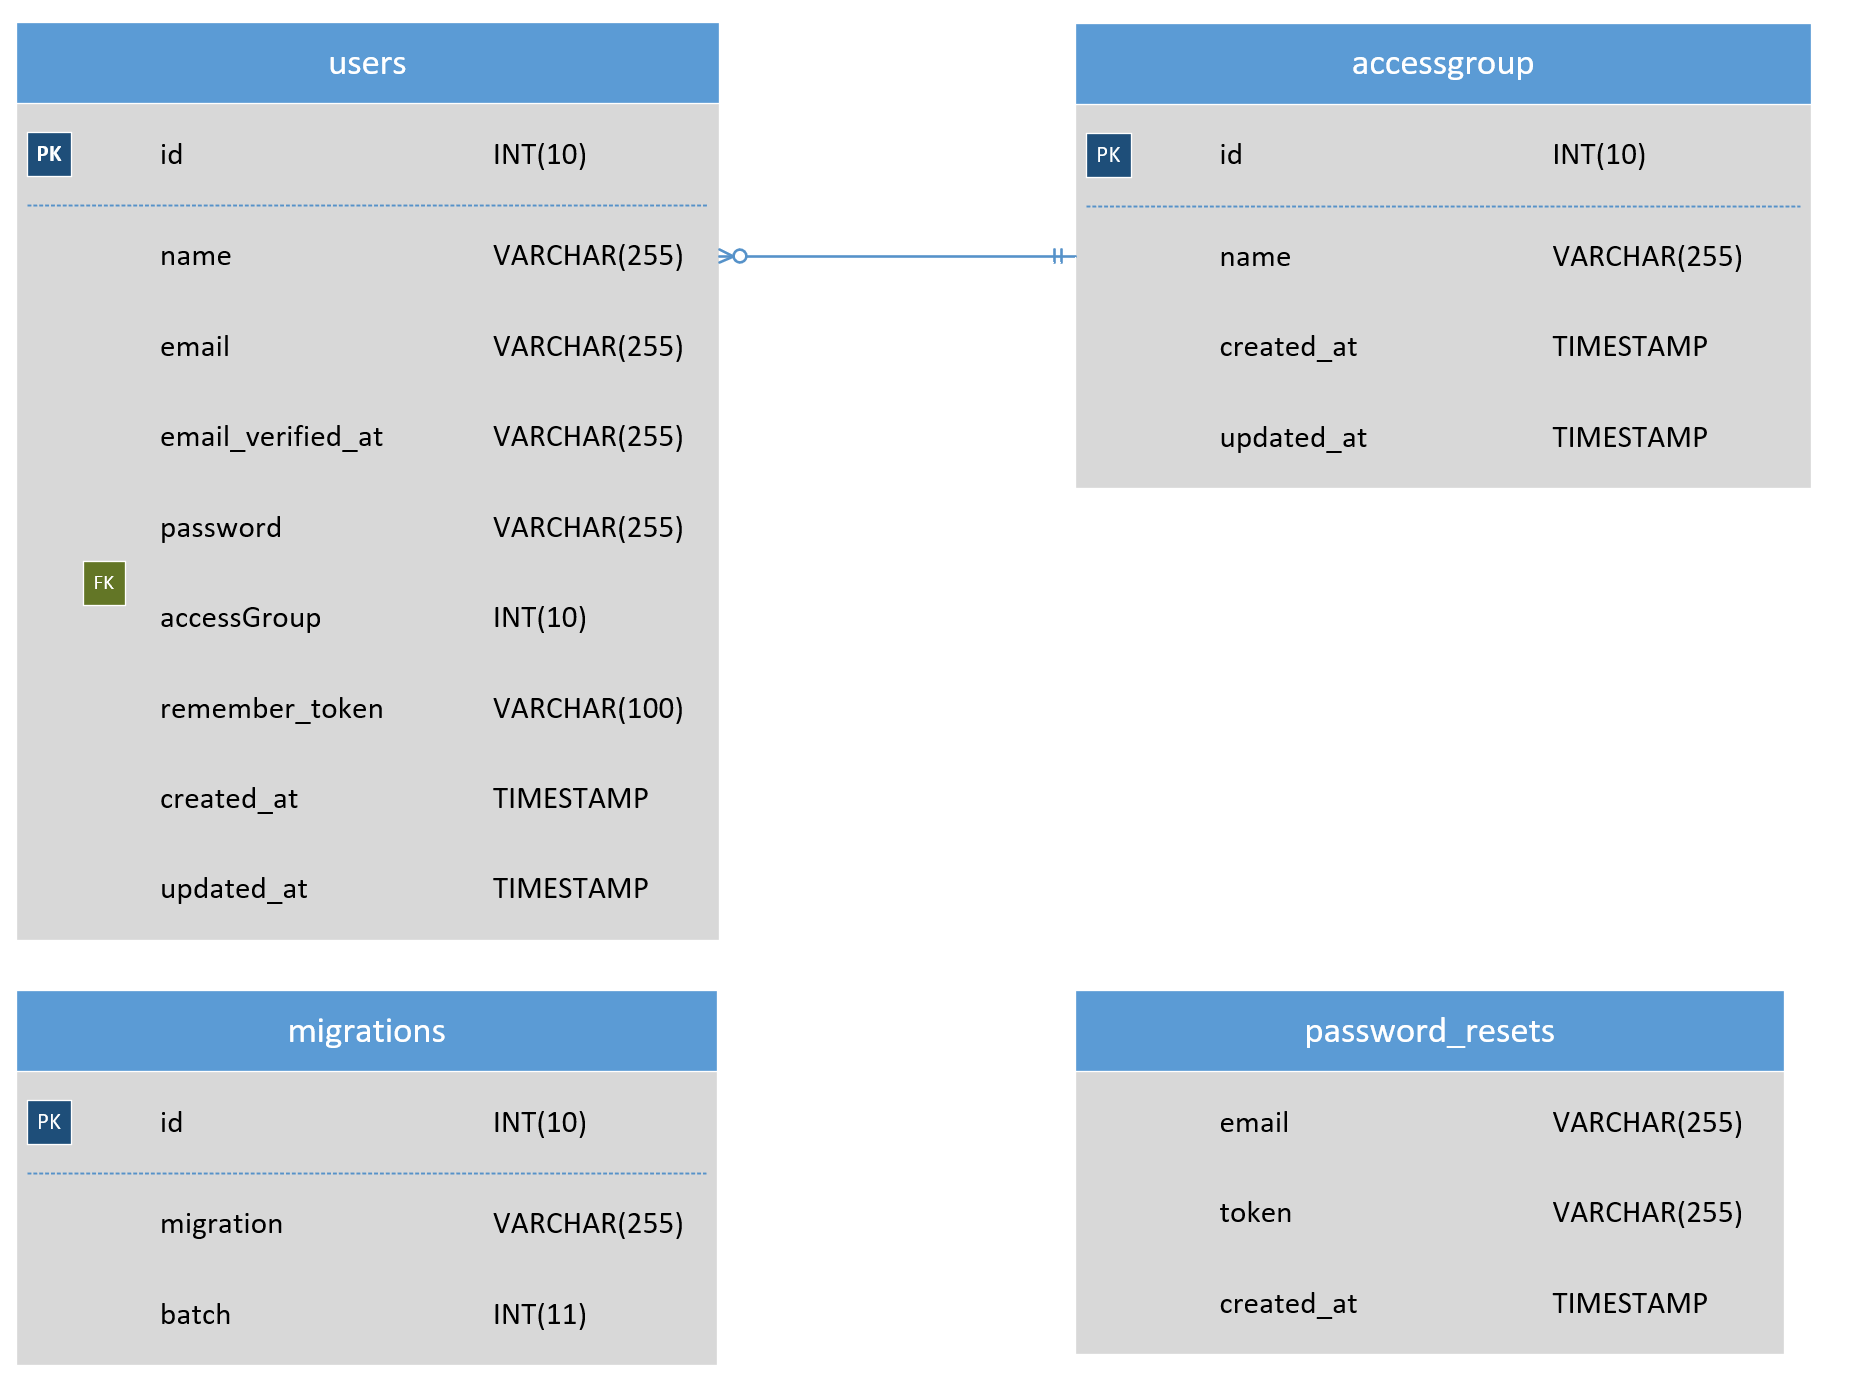
\includegraphics[scale=0.29]{db_schema1.png}
	\end{figure}
\end{frame}

\begin{frame}{Schema del database}
	\begin{figure}[!h]
		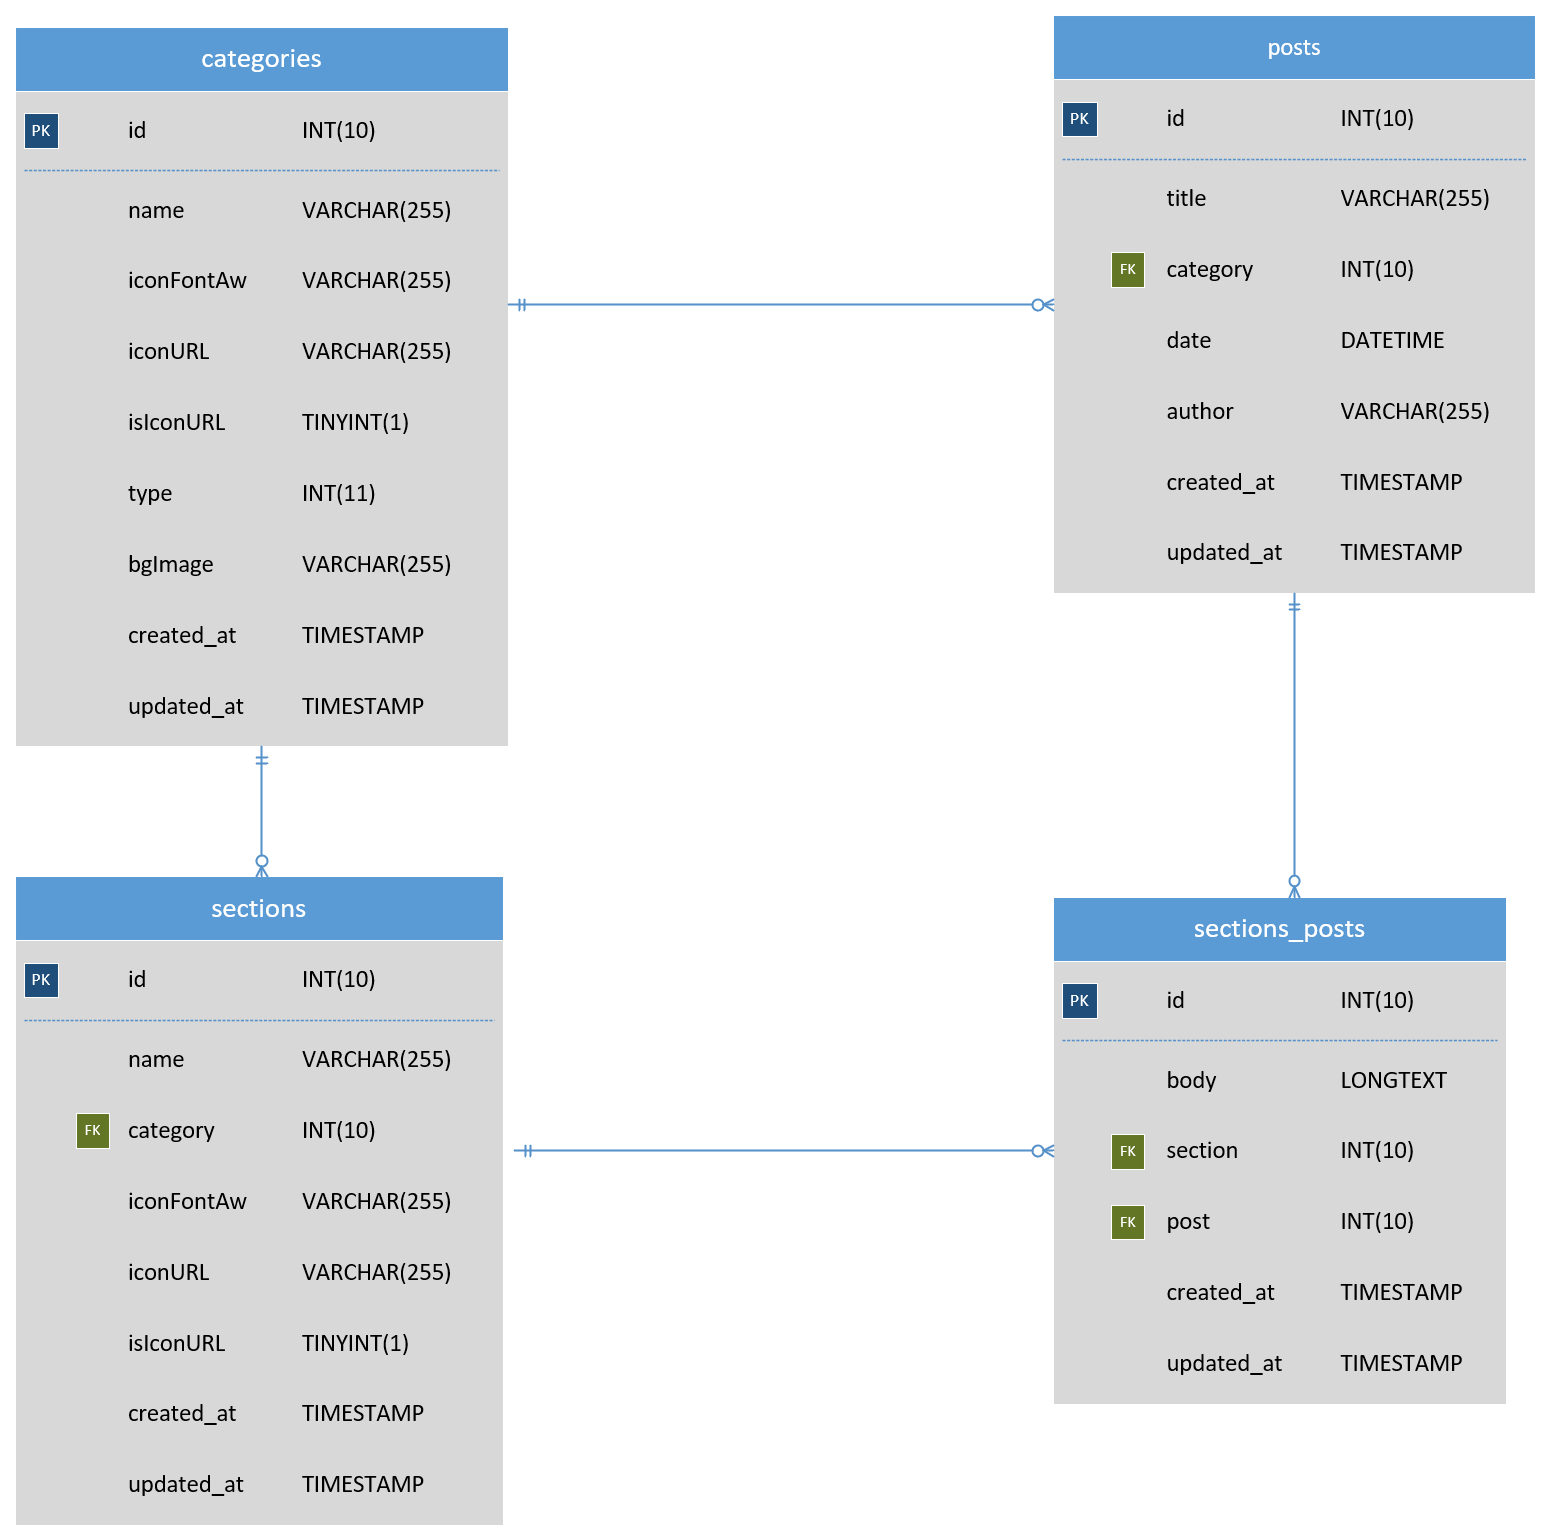
\includegraphics[scale=0.3]{db_schema2.png}
	\end{figure}
\end{frame}

\begin{frame}{Diagramma dei casi d'uso}
	\begin{figure}[!h]
		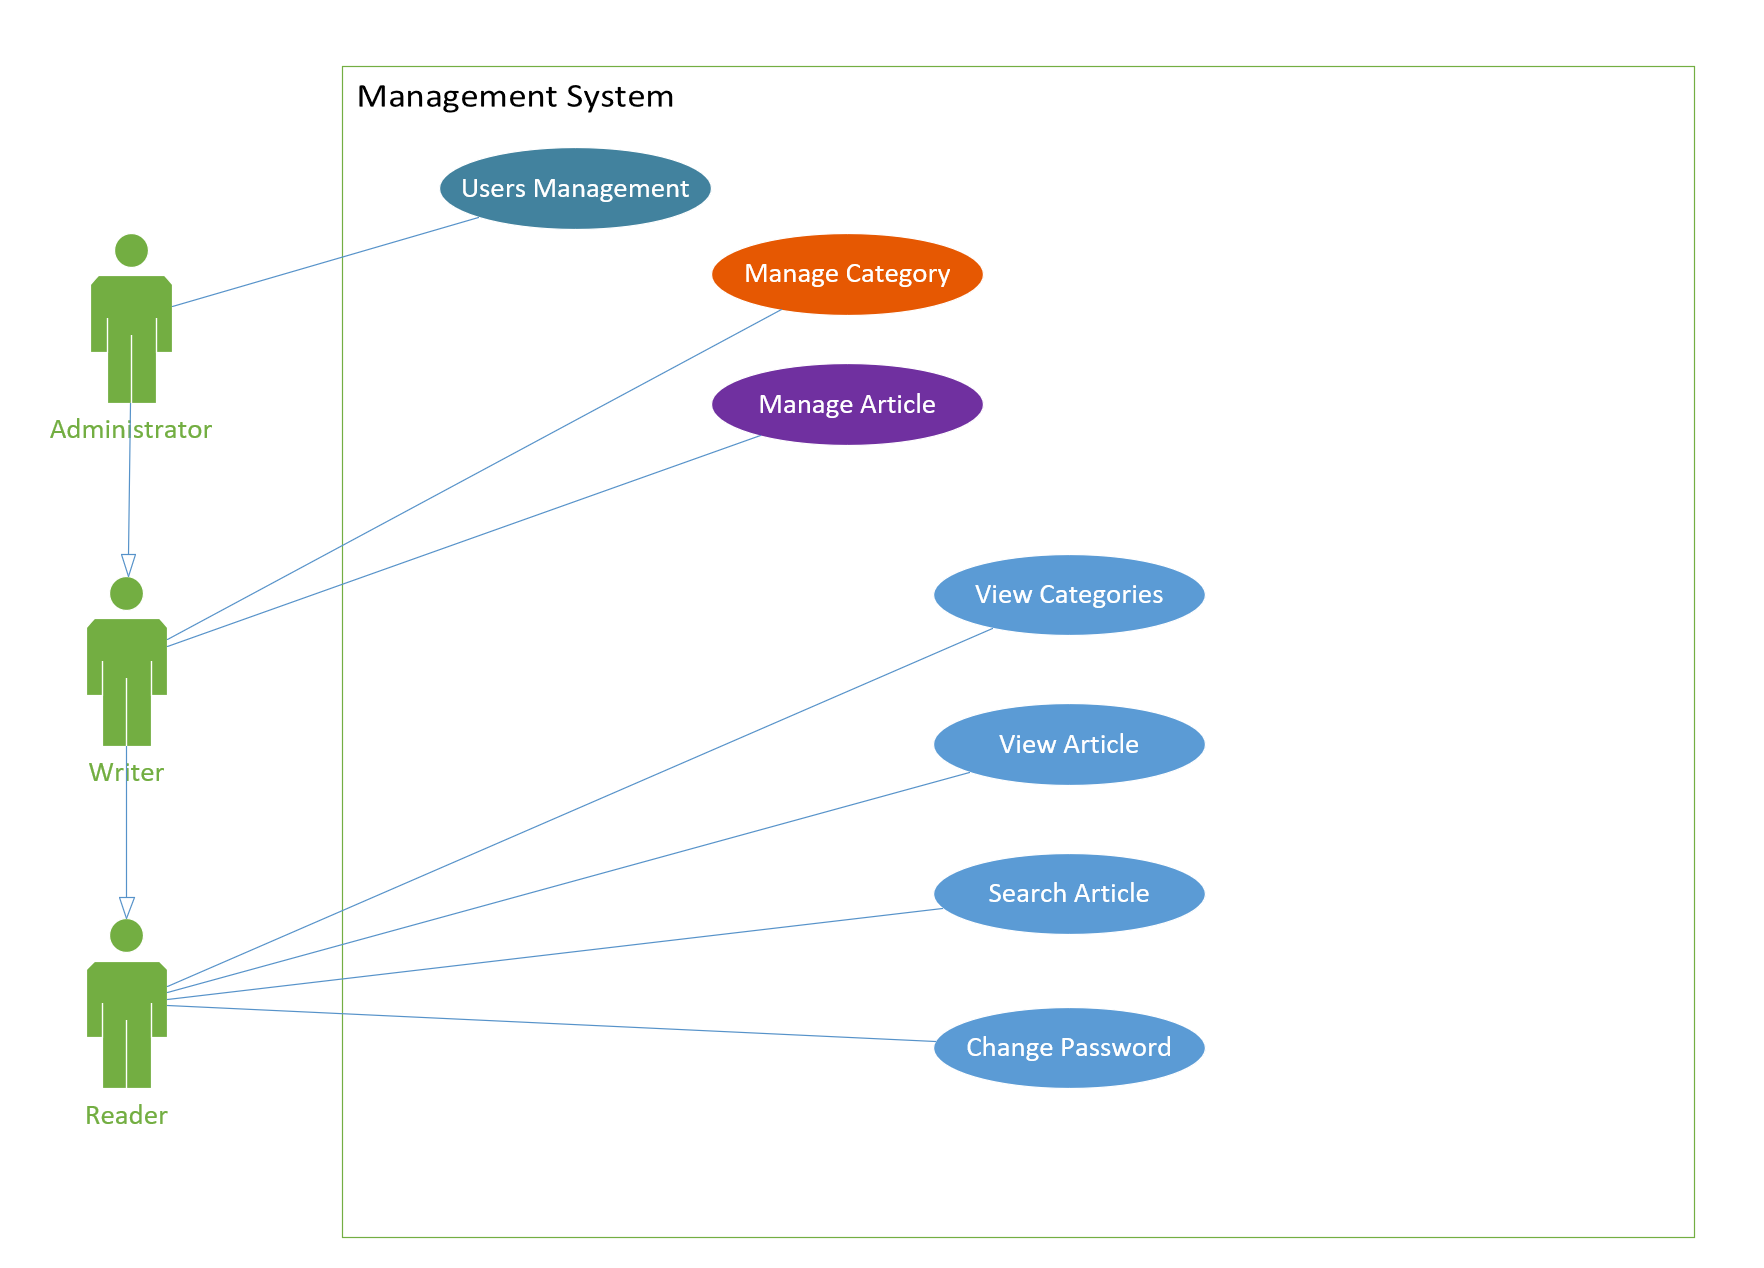
\includegraphics[scale=0.35]{uml_managementSystem.png}
	\end{figure}
\end{frame}

\begin{frame}{Diagramma dei casi d'uso}
	\begin{figure}[!h]
		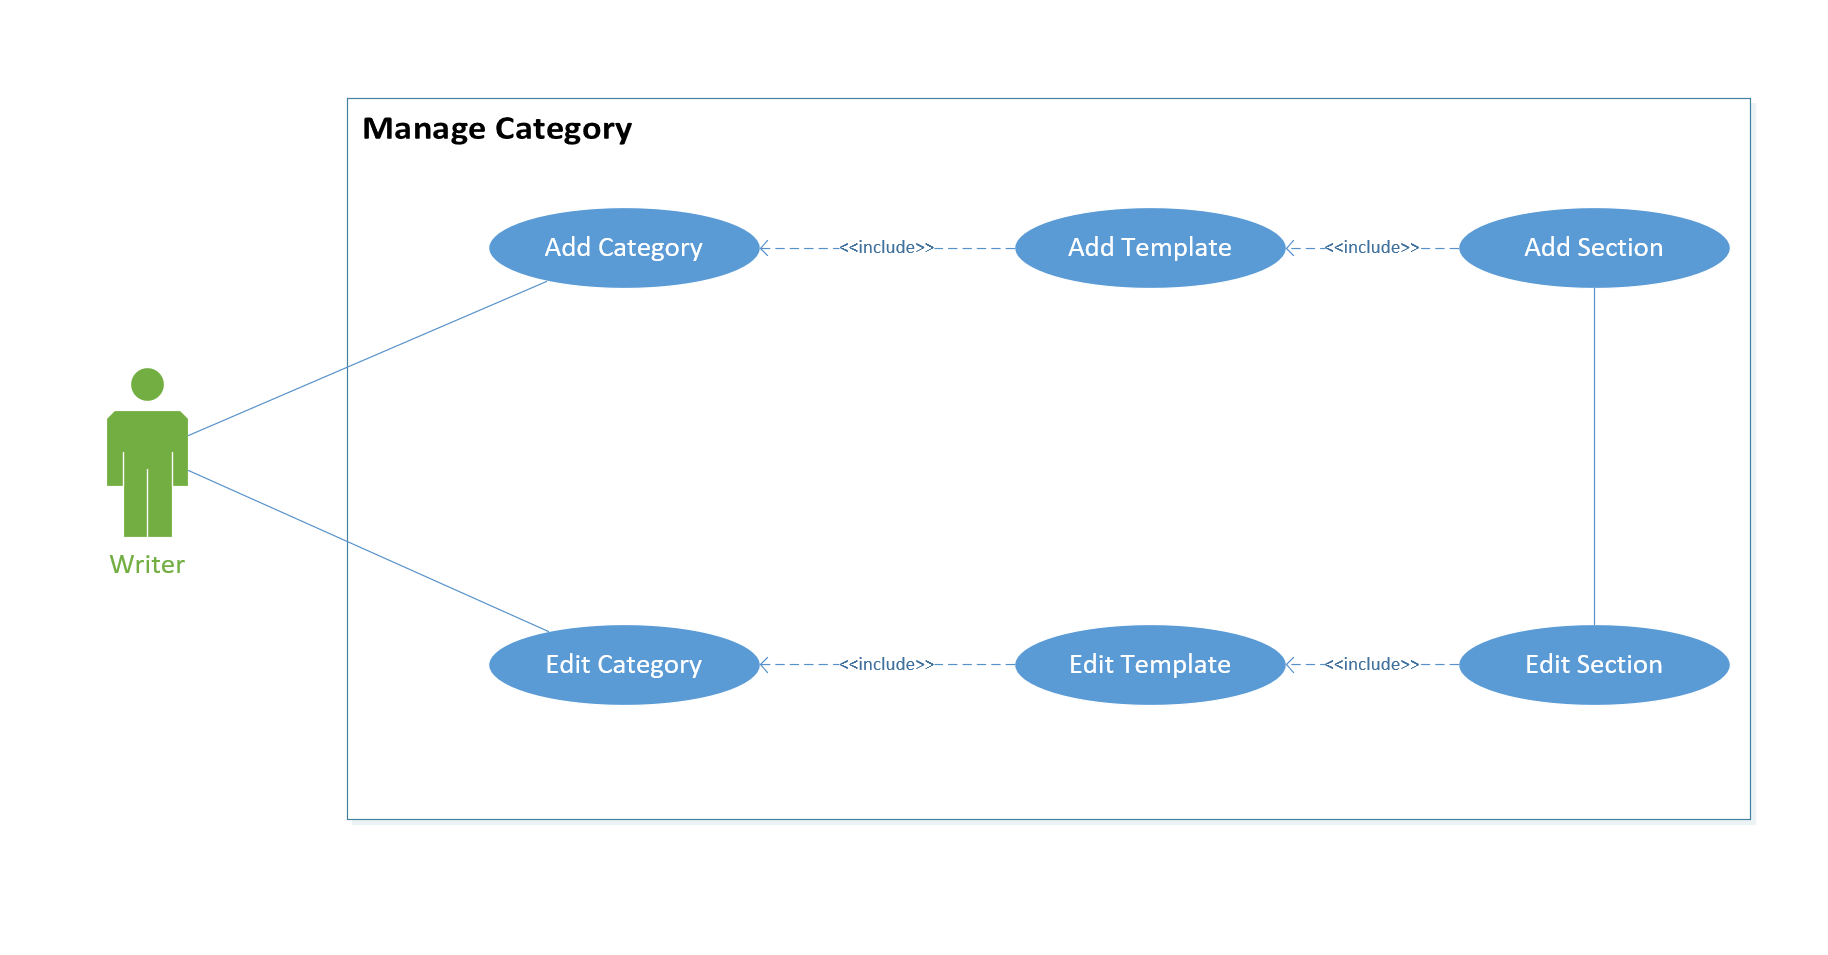
\includegraphics[scale=0.4]{uml_manageCategory.png}
	\end{figure}
\end{frame}
% --------------------------------------------------------------------------


\section{Implementazione}
\begin{frame}{Laravel - Pattern MVC}
\begin{columns}
	\column{1\textwidth}
	\begin{figure}[!h]
		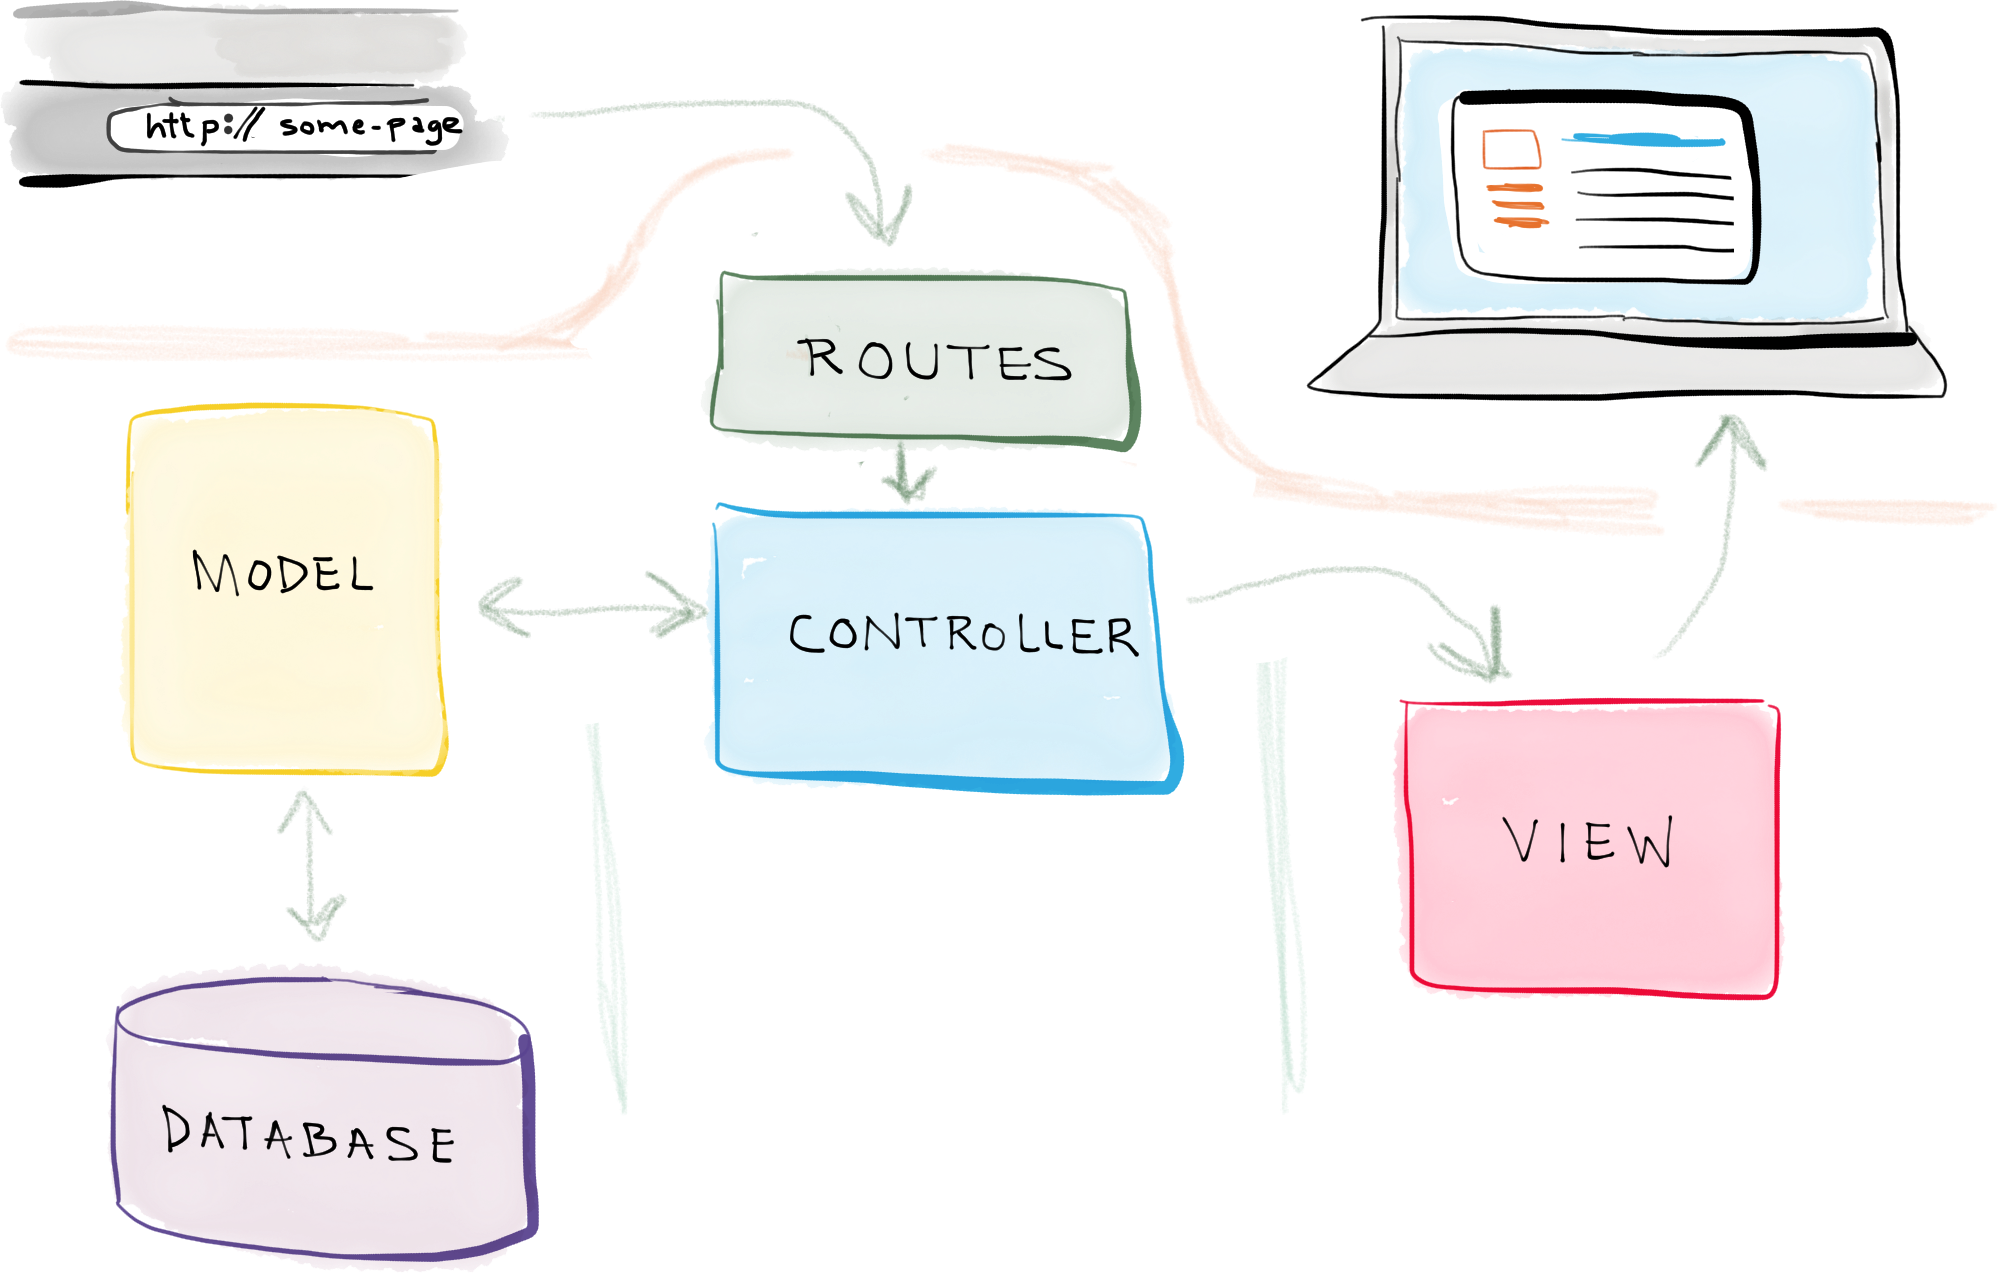
\includegraphics[scale=0.1]{mvc_diagram.png}
	\end{figure}
\end{columns}
\end{frame}

% --------------------------------------------------------------------------

\section{Demo}

% --------------------------------------------------------------------------

\section{Conclusioni}
\begin{frame}{Sviluppi futuri}
\begin{itemize}
	\item Caricamento dinamico di immagini, video e documenti sul server
	\item Certificato di sicurezza
	\item Integrazione con Ionic
	\item Sfondo diverso per ogni categoria
\end{itemize}
\end{frame}

% --------------------------------------------------------------------------
\begin{frame}[plain]

\end{frame}

\begin{frame}[plain]

\end{frame}

\begin{frame}{Login e sicurezza}
\begin{columns}
	\column{1\textwidth}
	\begin{figure}[!h]
		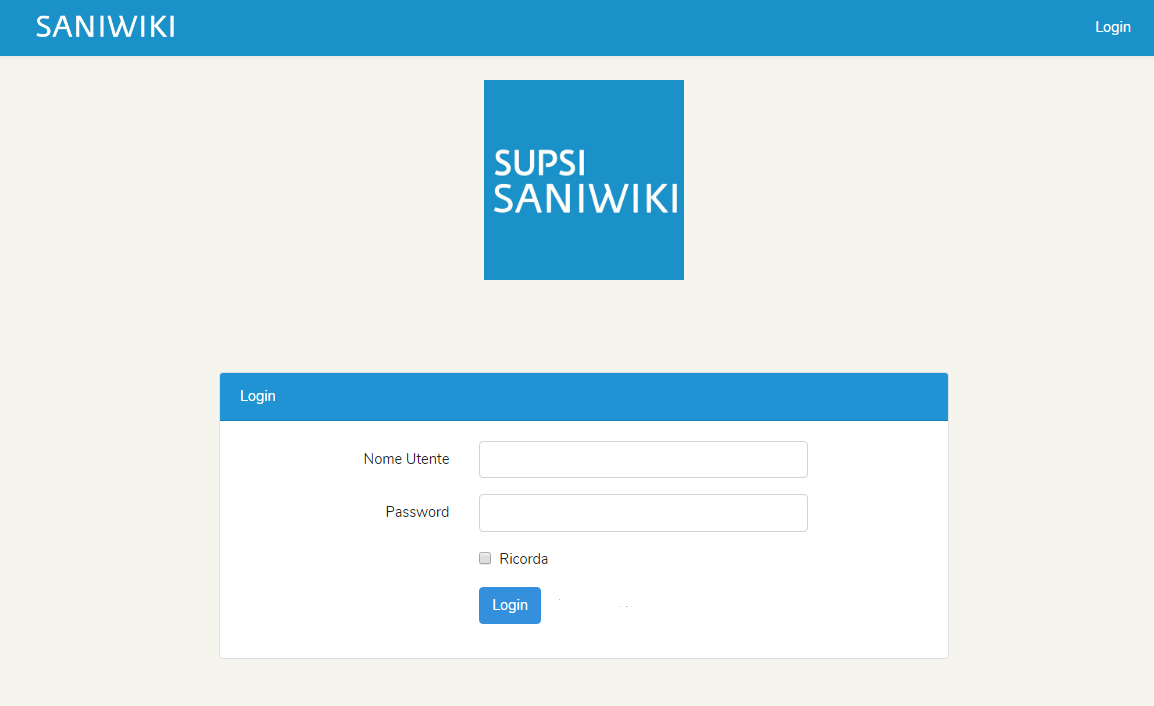
\includegraphics[scale=0.35]{saniwiki_login.png}
	\end{figure}
\end{columns}
\end{frame}

\begin{frame}{Gestione utenti}
\begin{columns}
	\column{1\textwidth}
	\begin{figure}[!h]
		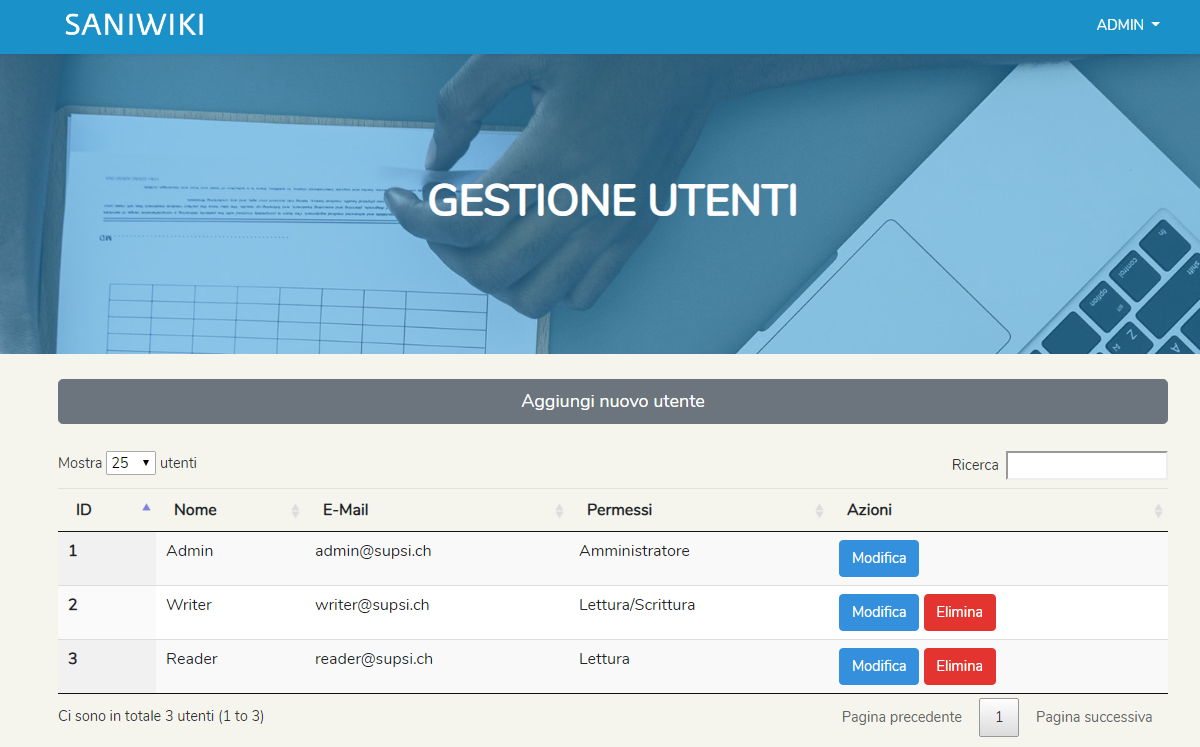
\includegraphics[scale=0.30]{saniwiki_gestioneutenti.png}
	\end{figure}
\end{columns}
\end{frame}

\begin{frame}[plain]{Vista principale}
\begin{columns}
	\column{1\textwidth}
	\begin{figure}[!h]
		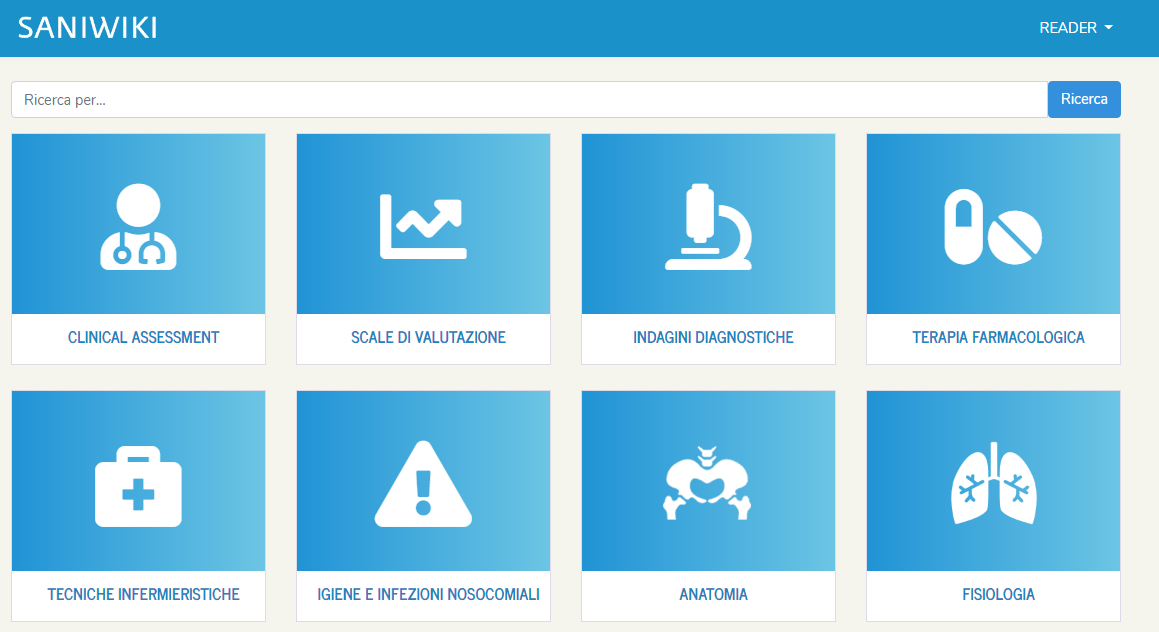
\includegraphics[scale=0.35]{saniwiki_categorie.png}
	\end{figure}
\end{columns}
\end{frame}

\begin{frame}[plain]{Vista degli articoli}
\begin{columns}
	\column{1\textwidth}
	\begin{figure}[!h]
		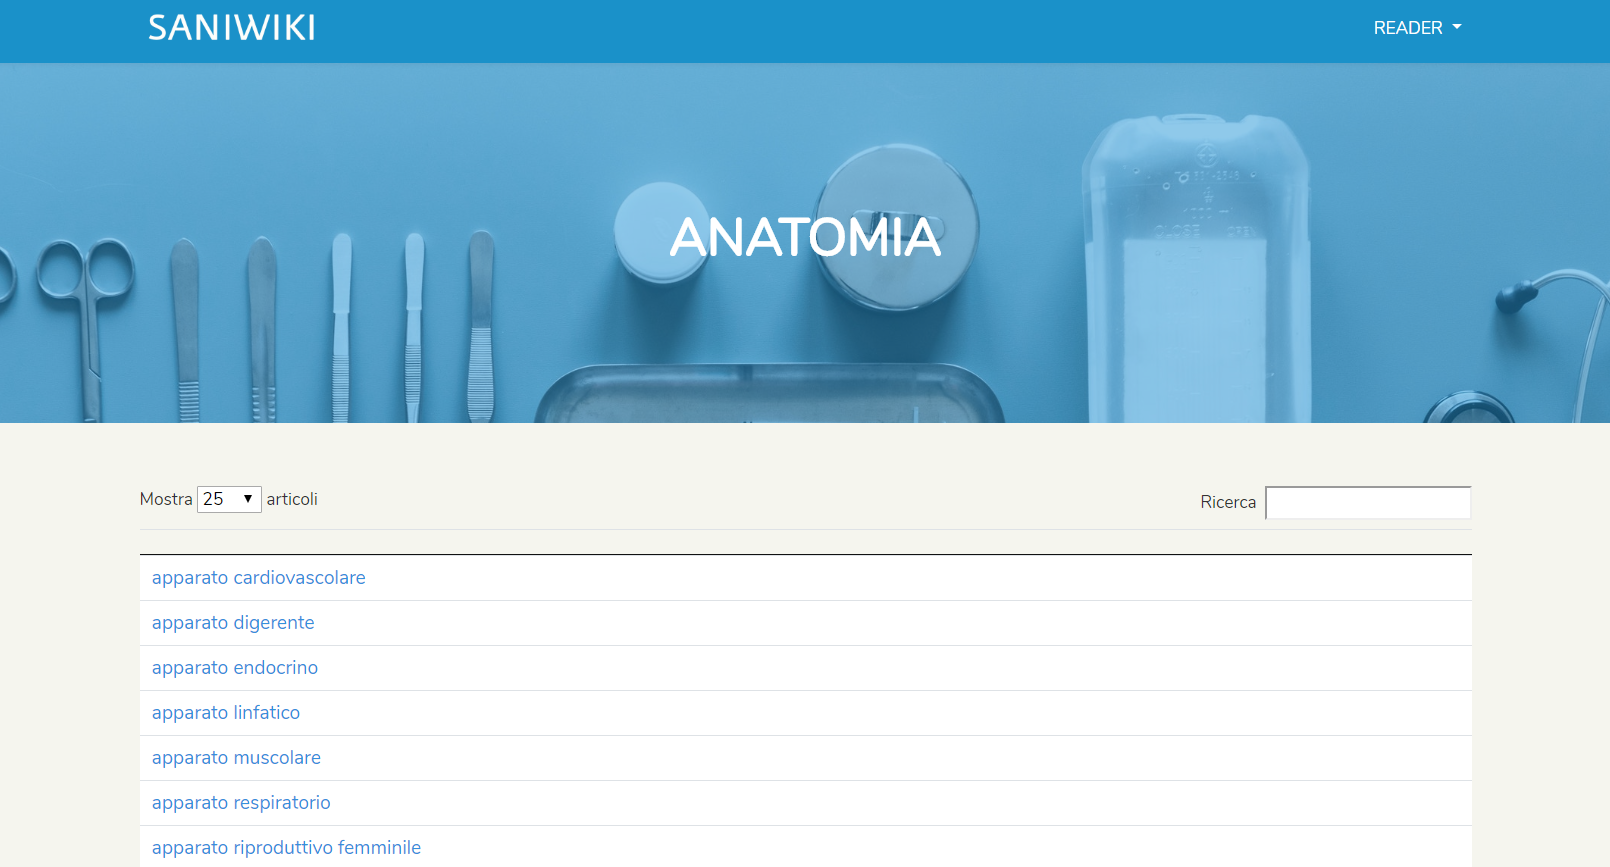
\includegraphics[scale=0.37]{saniwiki_articoli.png}
	\end{figure}
\end{columns}
\end{frame}

\begin{frame}[plain]{Lettura di un articolo}
\begin{columns}
	\column{1\textwidth}
	\begin{figure}[!h]
		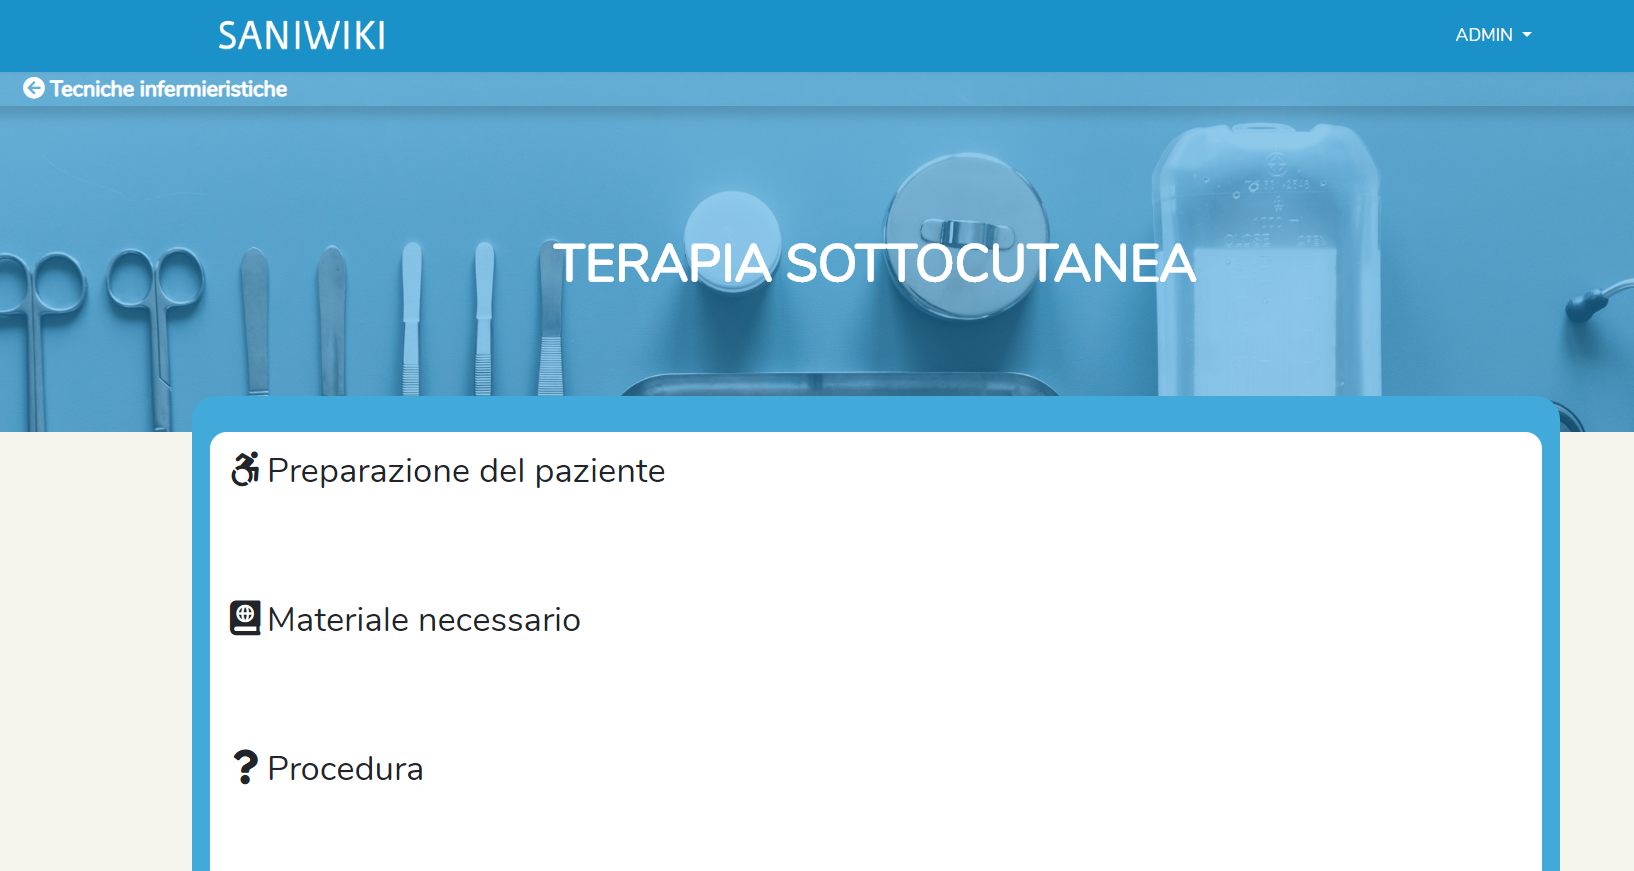
\includegraphics[scale=0.37]{saniwiki_sezioni.png}
	\end{figure}
\end{columns}
\end{frame}

\begin{frame}[plain]{Strumenti di scrittura}
\begin{columns}
	\column{.3\textwidth}
	\begin{figure}[!h]
		
\includegraphics[scale=0.3]{saniwiki_aggiungicategorie.png}
	\end{figure}
	\column{.7\textwidth}
	\begin{figure}[!h]
		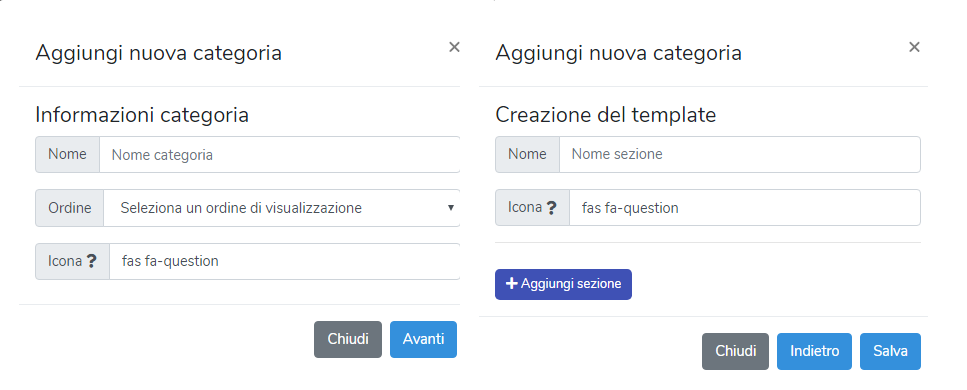
\includegraphics[scale=0.32]{saniwiki_aggiuntacategoria.png}
	\end{figure}
\end{columns}
\end{frame}

\begin{frame}[plain]{Strumenti di scrittura}
\begin{columns}
	\column{.3\textwidth}
	\begin{figure}[!h]
		
\includegraphics[scale=0.3]{saniwiki_modificaeliminacategoria.png}
	\end{figure}
	\column{.7\textwidth}
	\begin{figure}[!h]
		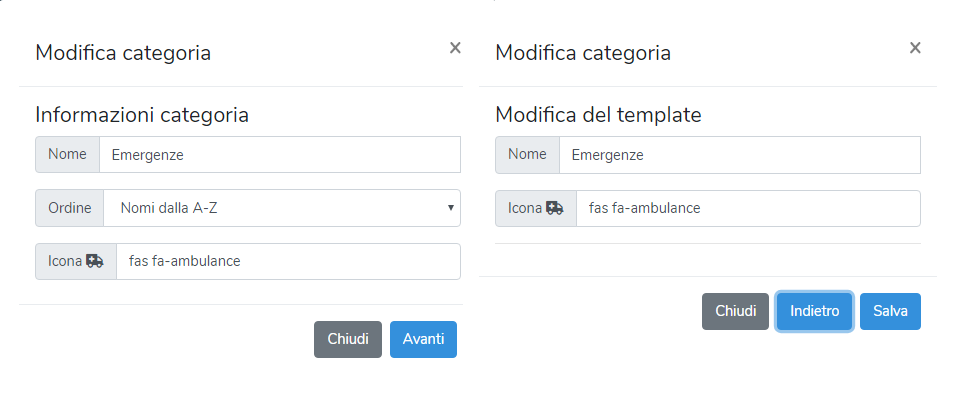
\includegraphics[scale=0.32]{saniwiki_modificacategoria.png}
	\end{figure}
\end{columns}
\end{frame}

\begin{frame}[plain]{Strumenti di scrittura}
\begin{columns}
	\column{.5\textwidth}
	\begin{figure}[!h]
		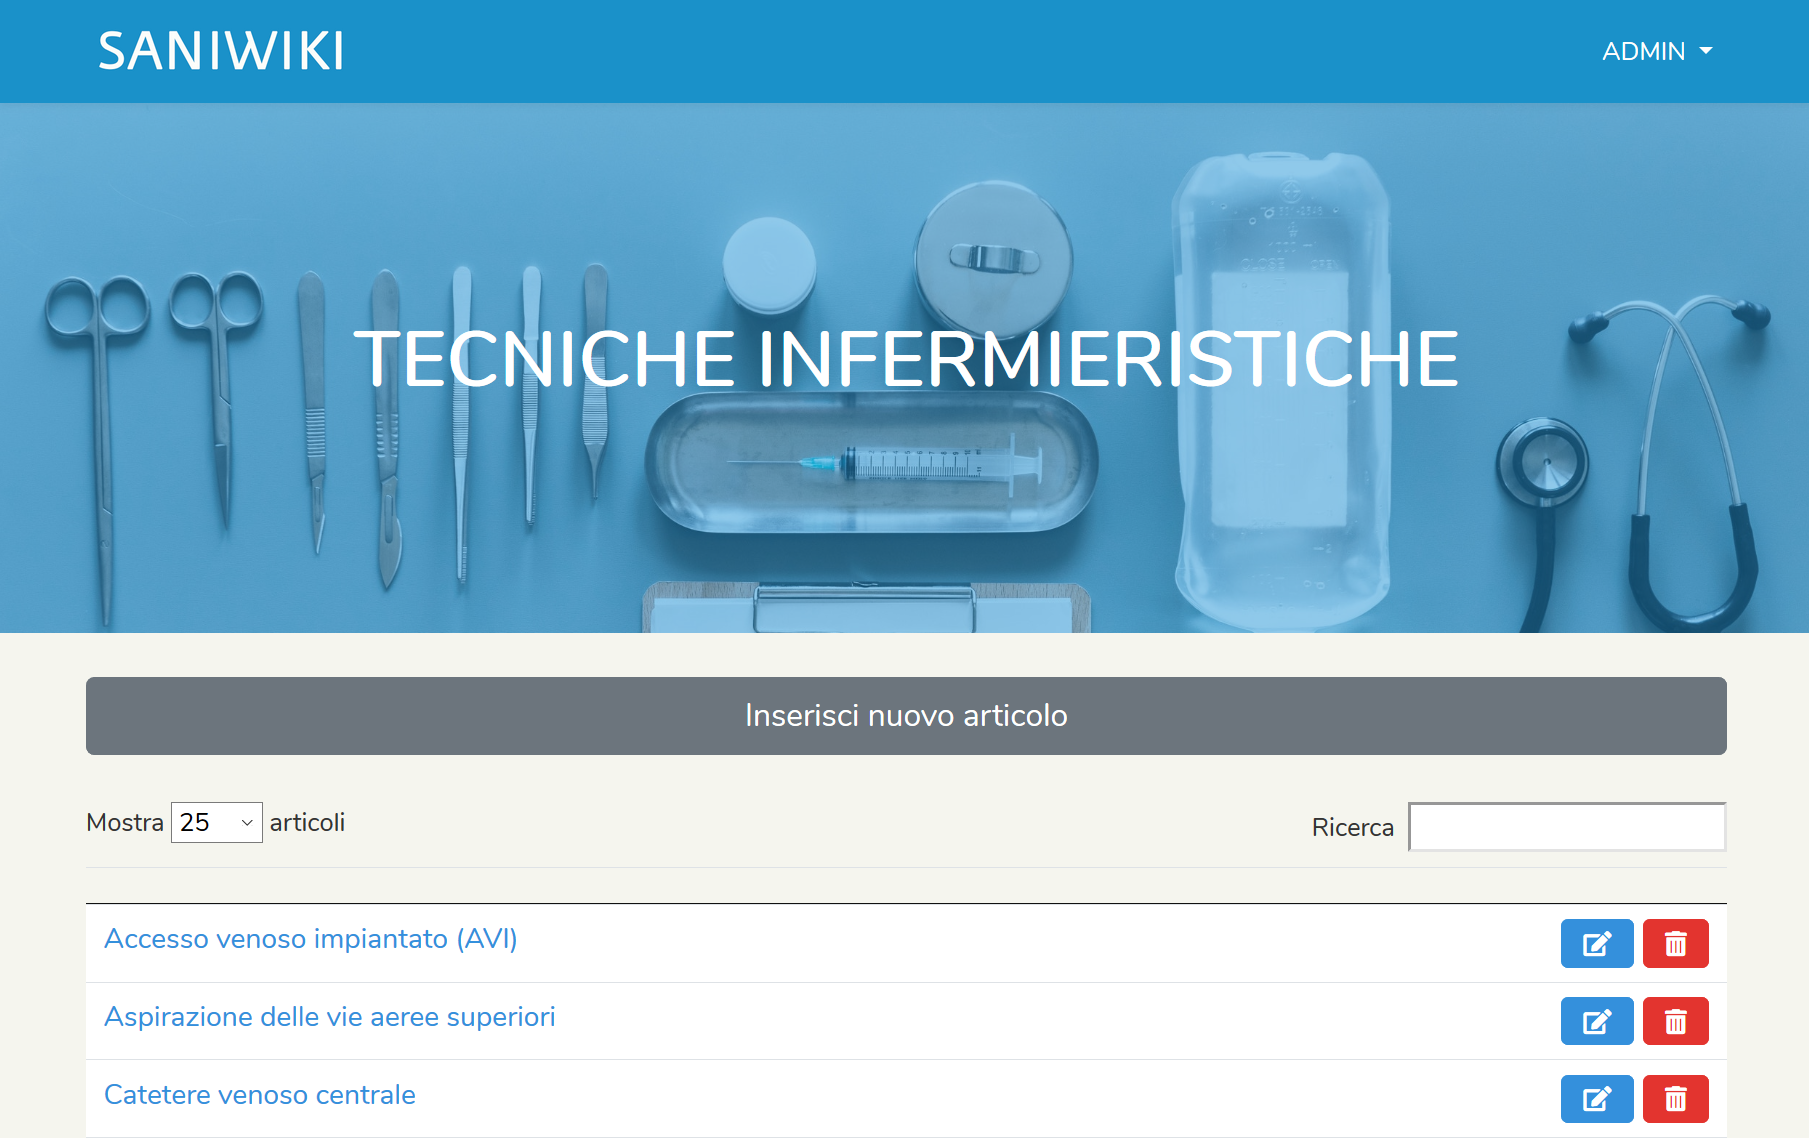
\includegraphics[scale=0.17]{saniwiki_modificaeliminaArticolo.png}
	\end{figure}
	\column{.5\textwidth}
	\begin{figure}[!h]
		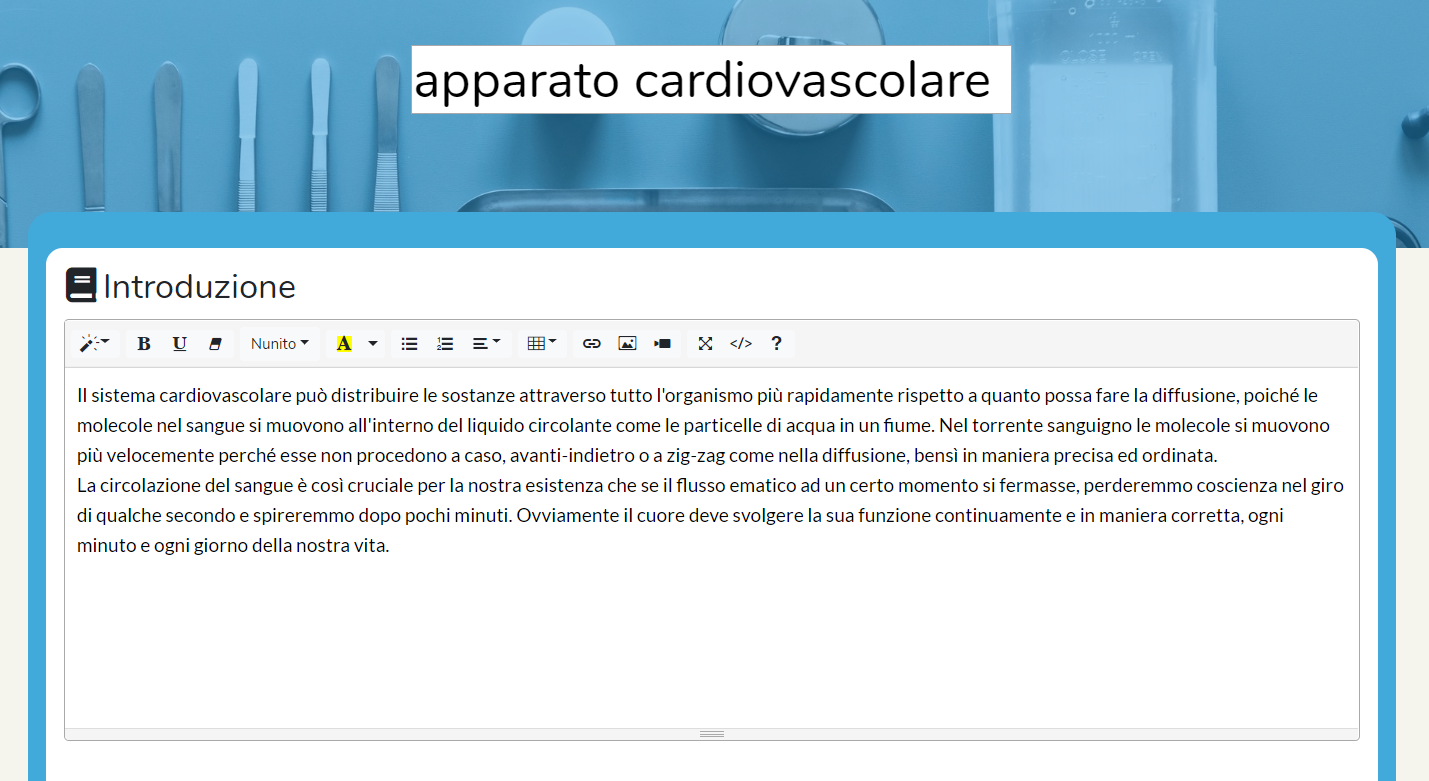
\includegraphics[scale=0.21]{saniwiki_modificaarticolo.png}
	\end{figure}
\end{columns}
\end{frame}

\end{document}